\section{Mục tiêu bài Lab 3}
Mục tiêu của Lab 3 tập trung vào các phương pháp Value-Based Reinforcement Learning nâng cao:
\begin{itemize}
    \item Hiểu bản chất của Bootstrapping trong Temporal Difference (TD) Learning.
    \item Phân biệt và triển khai các biến thể: TD(0), n-step TD, và Monte Carlo.
    \item Ứng dụng Function Approximation với Neural Network để giải quyết bài toán không gian trạng thái liên tục.
\end{itemize}

\subsection{3.1 Temporal Difference Learning (TD Learning)}
\textbf{Mô tả thực nghiệm:}
Chúng ta triển khai thuật toán TD(0) để học giá trị trạng thái $V(s)$ trên môi trường CartPole-v1. Vì CartPole có không gian liên tục, ta thực hiện rời rạc hóa (discretization) thành 1,600 trạng thái ($4 \times 4 \times 10 \times 10$). Kết quả được so sánh với Monte Carlo Prediction (được chạy 60,000 episodes để làm Ground Truth).

\begin{figure}[H]
    \centering
    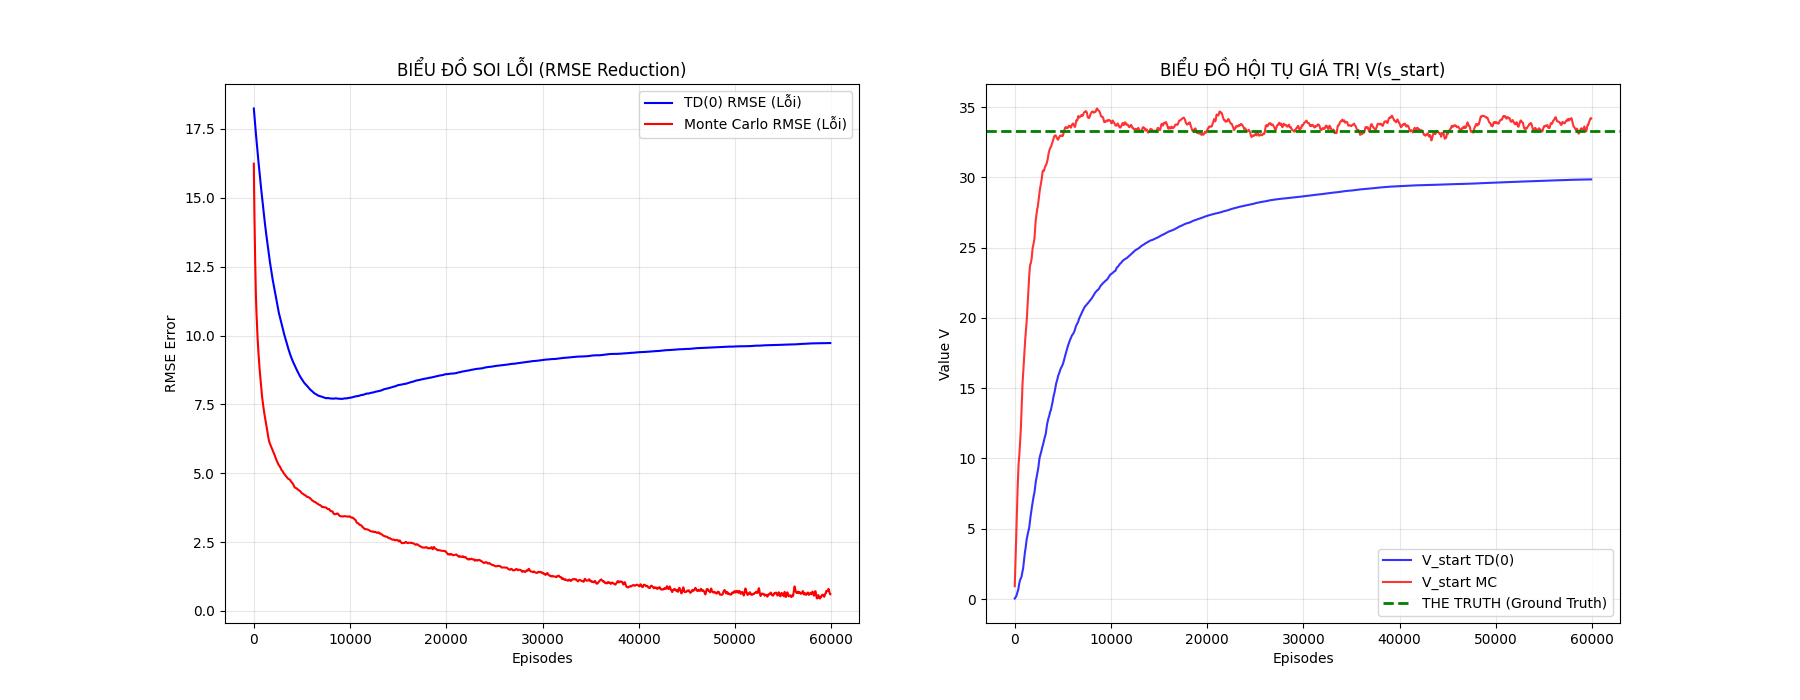
\includegraphics[width=0.9\textwidth]{Images/Lab3/stability_analysis.png}
    \caption{Phân tích độ ổn định và lỗi RMSE giữa TD(0) và Monte Carlo}
    \label{fig:lab3_td}
\end{figure}

\textbf{Nhận xét đồ thị (Hình \ref{fig:lab3_td}):}
\begin{itemize}
    \item \textbf{Đồ thị RMSE (trái) — Tốc độ học:} TD(0) có đường RMSE giảm nhanh và mượt mà hơn rõ rệt so với Monte Carlo trong các episode đầu tiên. Đây là hệ quả trực tiếp của Bootstrapping: TD(0) cập nhật $V(s)$ ngay sau mỗi bước đi (không cần chờ episode kết thúc), nên thông tin lan truyền nhanh hơn gấp nhiều lần so với MC vốn phải đợi đến cuối episode mới cập nhật toàn bộ.
    \item \textbf{Đồ thị RMSE (trái) — Mức nhiễu hội tụ:} Ở giai đoạn cuối, cả hai đều ổn định nhưng MC dao động nhiều hơn TD(0). Nguyên nhân là Variance của MC cao (tích lũy nhiễu từ toàn bộ chuỗi phần thưởng $G_t$), còn TD(0) chỉ phụ thuộc vào 1 bước nhiễu duy nhất ($r + \gamma V(s')$).
    \item \textbf{Đồ thị ổn định (phải):} Giá trị $V(s)$ của TD(0) ổn định quanh một mức nhất quán ngay từ sớm. Trong khi đó, Monte Carlo có biên độ dao động lớn hơn đáng kể vì mỗi episode lại cho một tổng thưởng $G_t$ khác nhau tùy vào kết quả ngẫu nhiên của toàn bộ chuỗi hành động.
\end{itemize}

\textbf{Trả lời câu hỏi lý thuyết:}
\begin{enumerate}
    \item \textbf{Bản chất của Bootstrapping:} TD(0) tận dụng tính đệ quy của \textbf{Phương trình Bellman} tối ưu. Việc cập nhật dựa trên giá trị của trạng thái kế tiếp được gọi là \textbf{Bootstrapping}. Về mặt lý thuyết, điều này cho phép thuật toán tận dụng cấu trúc Markov của môi trường để học hiệu quả từ dữ liệu trực tuyến (online) mà không cần hoàn tất quỹ đạo (trajectory).
    \item \textbf{So sánh TD(0) và Monte Carlo (MC):} MC cập nhật dựa trên tổng phần thưởng thực tế ($G_t$) cuối episode, còn TD cập nhật ngay lập tức sau mỗi bước dựa trên phần thưởng tức thời và giá trị dự đoán tiếp theo ($r + \gamma V(s')$). MC là phương pháp thống kê thuần túy, trong khi TD là phương pháp lặp (iterative) để giải hệ phương trình Bellman.
    \item \textbf{Phân rã Bias và Variance:} Đây là sự đánh đổi kinh điển trong học máy. MC là ước lượng \textbf{không chệch (unbiased)} vì nó sử dụng mẫu thực tế từ phân phối thực. Tuy nhiên, nó gặp vấn đề \textbf{phương sai cao (high variance)} do tích lũy nhiễu từ toàn bộ chuỗi hành động ngẫu nhiên. Ngược lại, TD(0) có \textbf{Bias cao} (phụ thuộc vào ước lượng ban đầu sai lệch) nhưng \textbf{Variance thấp} (chỉ phụ thuộc vào 1 bước nhiễu duy nhất), giúp quá trình hội tụ ổn định hơn trong các môi trường có tính ngẫu nhiên cao.
    \item \textbf{Tại sao TD phù hợp online?} Vì nó cập nhật theo từng bước (step-by-step), cho phép Agent học ngay trong khi đang tương tác mà không cần chờ episode kết thúc.
    \item \textbf{Ý nghĩa công thức TD(0):} $V(s) \leftarrow V(s) + \alpha [r + \gamma V(s') - V(s)]$. Trong đó $\alpha$ là tốc độ học, $r + \gamma V(s')$ là TD Target, và $r + \gamma V(s') - V(s)$ là TD Error.
    \item \textbf{Hệ quả của Learning rate:} Nếu $\alpha$ quá lớn, giá trị V sẽ dao động và khó hội tụ. Nếu $\alpha$ quá nhỏ, tốc độ học sẽ cực chậm.
    \item \textbf{Khi $\gamma \to 1$:} Agent sẽ coi trọng các phần thưởng trong tương lai xa tương đương với phần thưởng hiện tại, giá trị trạng thái sẽ lớn hơn và đại diện cho tổng thưởng dài hạn.
    \item \textbf{Cài đặt V(s) cho CartPole:} Sử dụng kỹ thuật rời rạc hóa (Discretization) để chia các biến liên tục thành các "thùng" (bins), biến mỗi tổ hợp thành một chỉ số trong mảng (Q-table).
    \item \textbf{Hàm update TD(0):} 
    \begin{lstlisting}[style=PythonStyle, caption={TD(0) Update Rule}]
# TD(0) Update: V(s) = V(s) + alpha * (reward + gamma * V(s') - V(s))
v_next = 0 if done else v_td[next_state_idx]
v_td[state_idx] += alpha * (reward + gamma * v_next - v_td[state_idx])
    \end{lstlisting}
    Dòng code này tính toán sai số giữa mục tiêu dự đoán ($r + \gamma V'$) và giá trị hiện tại, sau đó điều chỉnh một khoảng $\alpha$ để tiến gần mục tiêu hơn.
    \item \textbf{Discretize trong CartPole:} Chia 4 chiều quan sát ($x, \dot{x}, \theta, \dot{\theta}$) thành các khoảng cố định bằng `np.digitize` hoặc tính tỉ lệ theo `MIN/MAX\_VALS`.
    \item \textbf{So sánh tốc độ và ổn định:} TD(0) thường hội tụ nhanh hơn về mặt số lượng bước đi và ổn định hơn MC do phương sai thấp.
    \item \textbf{Thay đổi sai số:} Khi số episode tăng, RMSE giữa $V(s)$ và giá trị thực giảm dần theo dạng hàm mũ và ổn định tại một mức nhiễu thấp.
    \item \textbf{Xu hướng Learning Curve:} Đồ thị RMSE (Hình \ref{fig:lab3_td} trái) cho thấy TD(0) giảm lỗi nhanh hơn MC ở giai đoạn đầu.
    \item \textbf{TD(0) cho action-value?} Có thể, đó chính là thuật toán SARSA hoặc Q-learning.
    \item \textbf{Vấn đề Gán trách nhiệm (Credit Assignment Problem):} Trong các môi trường có phần thưởng thưa thớt (Sparse Reward), TD(0) gặp khó khăn lớn vì tín hiệu thưởng chỉ xuất hiện ở cuối. Do TD chỉ cập nhật lùi lại đúng 1 bước mỗi lần, thông tin về phần thưởng phải "thẩm thấu" dần qua hàng ngàn episode để truyền từ trạng thái kết thúc về các trạng thái ban đầu. Điều này giải thích tại sao đồ thị học thường có giai đoạn phẳng lì trước khi đột ngột tăng vọt.
\end{enumerate}

\subsection{3.2 n-step Q-learning}
\textbf{Mô tả thực nghiệm:}
Chúng ta triển khai n-step Q-learning để trung hòa ưu nhược điểm của TD(0) và Monte Carlo. Thí nghiệm thực hiện so sánh giữa $n=1$ (Q-learning thông thường), $n=3$ và $n=5$.

\begin{figure}[H]
    \centering
    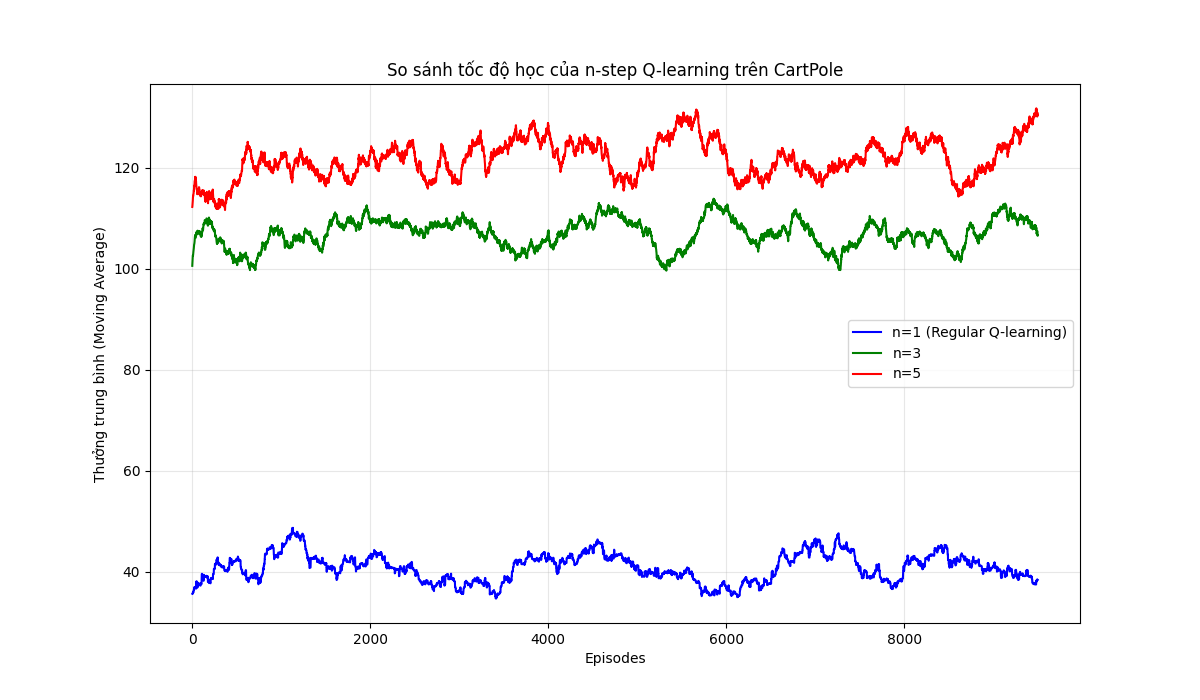
\includegraphics[width=0.8\textwidth]{Images/Lab3/n_step_comparison.png}
    \caption{So sánh tốc độ học của n-step Q-learning với các giá trị n khác nhau}
    \label{fig:lab3_nstep}
\end{figure}

\textbf{Nhận xét đồ thị (Hình \ref{fig:lab3_nstep}):}
\begin{itemize}
    \item \textbf{$n=1$ (TD thuần):} Đường Reward tăng chậm nhất. Vì mỗi bước cập nhật chỉ mang thông tin từ 1 phần thưởng tức thời $r_{t+1}$, tín hiệu học bị yếu và thông tin về đích phải lan truyền qua rất nhiều bước mới đến được các trạng thái ở xa — đây chính là hiện tượng Credit Assignment khó khăn.
    \item \textbf{$n=3$ và $n=5$ (n-step):} Đường Reward hội tụ nhanh hơn đáng kể và đạt mức cao hơn sớm hơn. Bằng cách tích lũy $n$ phần thưởng thực tế trước khi Bootstrapping, mỗi bước cập nhật mang thông tin phong phú hơn (giảm Bias so với $n=1$), giúp tín hiệu đích lan truyền nhanh hơn nhiều bước trong một lần cập nhật.
    \item \textbf{Tại sao không tăng n lên vô hạn?} Khi $n$ quá lớn, thuật toán tiến dần về Monte Carlo với Variance rất cao — đường Reward trở nên dao động mạnh và mất ổn định. Giá trị $n$ tối ưu là sự thỏa hiệp (Trade-off) giữa Bias thấp ($n$ lớn) và Variance thấp ($n$ nhỏ), thường nằm trong khoảng $n = 3 \sim 5$ với môi trường CartPole.
\end{itemize}

\textbf{Trả lời câu hỏi lý thuyết:}
\begin{enumerate}
    \item \textbf{Bản chất toán học:} n-step Q-learning đóng vai trò là một bộ lọc điều chỉnh sự đánh đổi giữa Bias và Variance. Nó học từ $n$ bước phần thưởng thực tế trước khi thực hiện bootstrapping, giúp giảm bớt sự lệ thuộc vào giá trị ước lượng ban đầu (giảm Approximation Bias).
    \item \textbf{Sự khác biệt về Return:} TD(0) chỉ sử dụng 1 reward tức thời, MC dùng toàn bộ quỹ đạo, còn n-step sử dụng một phần thực tế ($n$ rewards) kết hợp với giá trị dự đoán tại tương lai gần ($t+n$).
    \item \textbf{Phân rã Bias/Variance khi n tăng:} Khi $n$ tăng, Bias giảm (vì dùng nhiều dữ liệu thực hơn) nhưng Variance tăng (tích lũy nhiều nhiễu từ các hành động ngẫu nhiên trong chuỗi $n$ bước). Giá trị $n$ tối ưu là "điểm ngọt" giúp tối thiểu hóa tổng sai số bình phương (MSE).
    \item \textbf{Công thức n-step return:} $G_{t:t+n} = r_{t+1} + \gamma r_{t+2} + ... + \gamma^{n-1} r_{t+n} + \gamma^n \max_{a} Q(s_{t+n}, a)$.
    \item \textbf{Vai trò max Q:} Đại diện cho giá trị kỳ vọng tốt nhất mà Agent có thể đạt được từ trạng thái thứ $n$ trở đi.
    \item \textbf{Tối ưu hóa Credit Assignment:} n-step giúp giải quyết vấn đề gán trách nhiệm hiệu quả hơn. Vì mỗi bước cập nhật tác động ngược lại đến toàn bộ $n$ trạng thái trước đó, giúp tín hiệu phần thưởng từ đích (Goal) được truyền về nhanh hơn đáng kể so với TD(0).
    \item \textbf{Cấu trúc n-step buffer:} Sử dụng một hàng đợi (`deque`) lưu trữ các bộ $(s, a, r)$ có độ dài cố định là $n$.
    \item \textbf{Xử lý khi episode kết thúc sớm:} Nếu episode kết thúc tại bước $T < t+n$, ta tính n-step return dựa trên các phần thưởng thực tế còn lại và không thực hiện bootstrapping ($\gamma^n \max Q = 0$).
    \item \textbf{Hàm tính n-step return:} Duyệt qua buffer, nhân mỗi reward với $\gamma^i$ tương ứng.
    \begin{lstlisting}[style=PythonStyle, caption={n-step Return Calculation}]
# Calculate n-step return G: r_t + gamma*r_{t+1} + ... + gamma^{n-1}*r_{t+n-1}
G = 0
for i, (_, _, r_i) in enumerate(buffer):
    G += (gamma ** i) * r_i
# Bootstrapping term: gamma^n * max Q(s_{t+n})
if not done:
    G += (gamma ** len(buffer)) * np.max(q_table[state_idx])
# Update rule
q_table[s_t, a_t] += alpha * (G - q_table[s_t, a_t])
    \end{lstlisting}
    \item \textbf{So sánh n=1, 3, 5:} Thường $n=3$ hoặc $n=5$ cho kết quả tốt nhất (Hình \ref{fig:lab3_nstep}) vì tận dụng được thông tin reward dài hơn mà không bị quá nhiễu.
    \item \textbf{Khi n quá lớn:} Thuật toán mất dần tính chất Bootstrapping và tiến dần về Monte Carlo, dẫn đến Variance cực cao và làm quá trình học mất ổn định do nhiễu tích lũy.
    \item \textbf{Tăng tốc độ hội tụ (Convergence Rate):} n-step thường hội tụ nhanh hơn về mặt thời gian thực vì nó tận dụng được nhiều thông tin hơn trong mỗi lần cập nhật trọng số.
    \item \textbf{Chiến lược chọn n:} Ta nên chọn $n$ nhỏ cho môi trường có độ bất định cao (stochastic) để giữ variance thấp, và chọn $n$ lớn cho môi trường ổn định hoặc có phần thưởng thưa (sparse reward) để tăng tốc độ lan truyền tín hiệu.
    \item \textbf{Episode dài:} n-step rất phù hợp vì giúp đẩy nhanh tốc độ hội tụ mà không cần chờ đến cuối episode như MC.
\end{enumerate}

\subsection{3.3 Q-function Approximation với Neural Network}
\textbf{Mô tả thực nghiệm:}
Triển khai mạng Neural Network (Deep Q-Network - DQN) sử dụng PyTorch để thay thế Q-table. Chúng ta sử dụng kiến trúc 3 lớp Fully Connected với hàm kích hoạt ReLU, kết hợp Replay Buffer và kỹ thuật Double DQN để ổn định quá trình huấn luyện.

\begin{figure}[H]
    \centering
    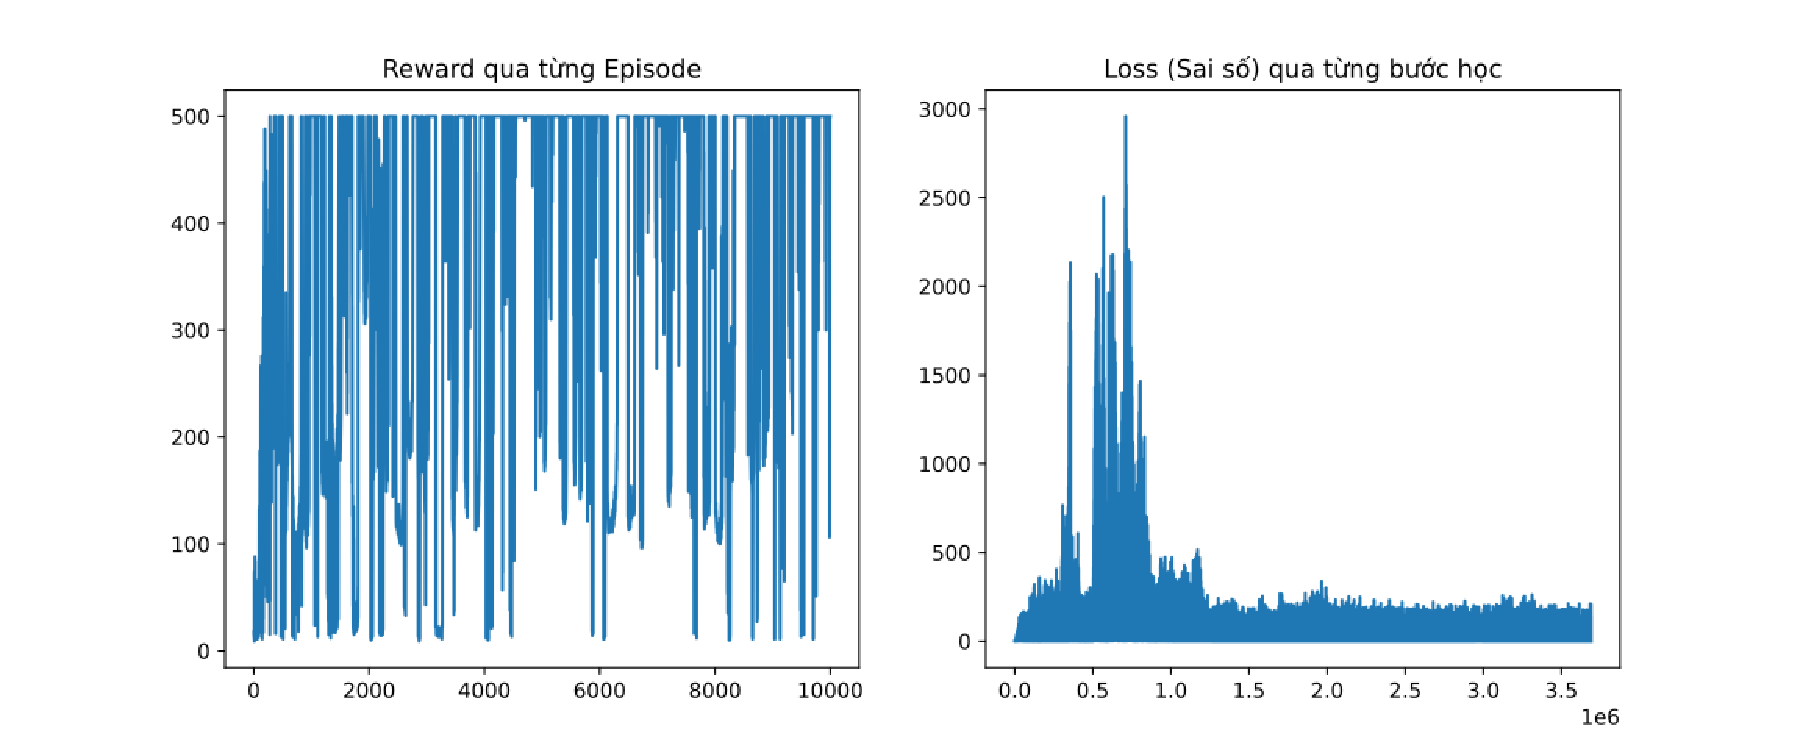
\includegraphics[width=1.0\textwidth]{Images/Lab3/deepRL-reward.pdf}
    \caption{Đồ thị Reward và Loss của mô hình DQN trên CartPole-v1}
    \label{fig:lab3_dqn}
\end{figure}

\textbf{Nhận xét đồ thị:}
Quan sát đồ thị Reward (trái) và Loss (phải), ta thấy cả hai đều có xu hướng dao động mạnh (oscillation) thay vì tăng/giảm đơn điệu và ổn định. Đây là hiện tượng đặc trưng của DQN và xuất phát từ sự tương tác của ba yếu tố chính:

\begin{itemize}
    \item \textbf{Replay Buffer gây tương quan dữ liệu (Correlated Samples):} Replay Buffer lưu lại các bộ $(s, a, r, s')$ từ các episode trước. Ở giai đoạn đầu, buffer chứa phần lớn các mẫu từ Policy kém (Agent chưa biết gì), khiến mạng liên tục học trên dữ liệu chất lượng thấp và Reward không thể tăng ổn định. Khi Policy được cải thiện và buffer dần được lấp đầy bằng các mẫu tốt hơn, Reward mới có xu hướng tăng dần. Tuy nhiên, nếu một mini-batch ngẫu nhiên lấy trúng nhóm mẫu xấu cũ, Reward lại tụt xuống ngay lập tức.

    \item \textbf{Learning Rate ($\alpha$) tạo dao động quanh điểm tối ưu:} Learning Rate kiểm soát bước nhảy của Gradient Descent. Nếu $\alpha$ quá lớn, mỗi bước cập nhật trọng số sẽ vượt qua điểm tối ưu (overshoot), khiến Loss không giảm mà còn có thể tăng trở lại ở bước tiếp theo. Trong đồ thị Loss (phải), các đột biến tăng vọt bất thường chính là biểu hiện của hiện tượng overshoot này. Về mặt toán học, đây chính là sự bất ổn định của Gradient Descent khi bước nhảy quá lớn so với độ cong (curvature) của hàm Loss.

    \item \textbf{Batch Size nhỏ làm tăng Gradient Noise:} Mỗi lần cập nhật mạng, ta chỉ lấy một mini-batch nhỏ (ví dụ 64 mẫu) thay vì toàn bộ dữ liệu. Gradient tính được từ 64 mẫu là một \textbf{ước lượng nhiễu} (noisy estimate) của Gradient thực. Điều này khiến hướng cập nhật trọng số không hoàn toàn chính xác ở mỗi bước, dẫn đến quỹ đạo học "lắc lư" xung quanh điểm hội tụ thay vì đi thẳng vào đó.
\end{itemize}

\textbf{Xu hướng tổng thể:} Mặc dù dao động mạnh ở từng episode, đường Reward trung bình (moving average) vẫn có xu hướng \textbf{tăng dần theo thời gian}, chứng tỏ mạng DQN vẫn đang học được Policy tốt hơn. Tương tự, đường Loss tuy có nhiều đột biến cục bộ nhưng nhìn tổng thể vẫn có xu hướng \textbf{ổn định ở mức thấp hơn}, đặc biệt ở các episode cuối — đây là dấu hiệu của quá trình hội tụ thành công.

\textbf{Trả lời câu hỏi lý thuyết:}
\begin{enumerate}
    \item \textbf{Lời nguyền đa chiều (Curse of Dimensionality):} Q-table không phù hợp vì số lượng trạng thái bùng nổ lũy thừa theo số chiều quan sát. Với CartPole (4 chiều liên tục), việc rời rạc hóa dù chỉ 10 mức mỗi chiều cũng tạo ra $10^4$ trạng thái; trong các bài toán thực tế phức tạp hơn, con số này trở nên bất khả thi để lưu trữ và khám phá. Ngoài ra, Q-table thiếu khả năng \textbf{Tổng quát hóa (Generalization)} — việc học tại một trạng thái không mang lại lợi ích cho các trạng thái lân cận có tính chất tương tự.
    \item \textbf{Ý tưởng Function Approximation:} Thay vì lưu giá trị cho từng ô, ta học một hàm số $Q(s, a; \theta)$ có khả năng dự đoán giá trị Q cho bất kỳ trạng thái nào dựa trên các tham số $\theta$.
    \item \textbf{Khác biệt Q-table vs Q-network:} Q-table là một mảng tra cứu tĩnh, Q-network là một mô hình toán học có khả năng học các đặc trưng và tổng quát hóa.
    \item \textbf{Kiến trúc mạng:} Input là vector trạng thái (4 chiều), qua các lớp ẩn (64 nodes) dùng ReLU, Output là giá trị Q của 2 hành động.
    \item \textbf{Tại sao Output node = số action?} Để trong một lần truyền xuôi (forward pass), mạng có thể tính toán đồng thời giá trị của tất cả các hành động khả thi tại trạng thái đó.
    \item \textbf{Vai trò ReLU:} Thêm tính phi tuyến (non-linearity) vào mạng, giúp nó xấp xỉ được các hàm số phức tạp thay vì chỉ là các đường thẳng.
    \item \textbf{Hàm loss:} Sử dụng Mean Squared Error (MSE) giữa giá trị dự đoán hiện tại $Q(s, a)$ và mục tiêu Bellman $r + \gamma \max Q(s', a')$.
    \item \textbf{Tại sao target có max Q?} Dựa trên phương trình Bellman tối ưu, khẳng định giá trị của trạng thái hiện tại bằng phần thưởng hiện tại cộng với giá trị tốt nhất có thể đạt được ở tương lai.
    \item \textbf{Target thay đổi quá nhanh:} Dẫn đến hiện tượng đuổi theo mục tiêu di động (moving target), làm quá trình huấn luyện mất ổn định. Để khắc phục, ta dùng Target Network (cập nhật chậm hơn).
    \item \textbf{Quan sát đồ thị Loss:} Model học tốt khi Loss giảm dần và ổn định ở một mức thấp (Hình \ref{fig:lab3_dqn} phải).
    \item \textbf{Quan sát Reward:} Agent đạt policy tốt khi đường Reward tăng dần và tiệm cận mức tối đa của môi trường (500 điểm cho CartPole-v1).
\end{enumerate}
